% Provenance (never printed): see sources/outline_sources.md (Year 1: stress and
% principal stresses in 2D; strain; pure and simple shear; elastic, brittle and ductile
% behaviour; the strength envelope of the lithosphere). Strength envelopes from
% figdata/bachelor-1/strength_envelope.py (Byerlee 1975; flow laws of Gleason and Tullis
% 1995 and Hirth and Kohlstedt 2003 as compiled by Lopez-Sanchez; geotherms of ch. 10);
\chapter{Esfuerzo, deformación y reología}\label{ch:b1:stress-strain-rheology}

En los años 1960, agua residual inyectada por un pozo de eliminación en el Rocky Mountain Arsenal, cerca de Denver, se difundió por el basamento
cristalino fracturado entre \qty{3.7}{km} y \qty{7.0}{km} bajo la superficie, y siguieron los terremotos. Se produjeron dentro de la parte de la roca
donde la presión del fluido había subido más de unos \qty{3.2}{MPa}.
% ledger: hb81:denver
Medio siglo después ocurrió lo mismo a mayor escala en Oklahoma, donde el agua salada extraída junto con el petróleo y el gas se vuelve a bombear bajo
tierra. En el estado y alrededores, los terremotos de magnitud 3 o mayor fueron de uno a cinco al año entre 2005 y 2008, luego \num{20} en 2009,
\num{585} en 2014 y \num{888} en 2015, más de dos al día; sacudidas de magnitud 5.7 y 5.8 estremecieron Prague, en 2011, y Pawnee, en 2016. Cuatro pozos
de gran volumen podían explicar por sí solos una quinta parte de los terremotos del centro de Estados Unidos, y provocar algunos a más de \qty{30}{km}
de distancia.
% ledger: usgs:oklahoma-rate, usgs:prague-pawnee, keranen:oklahoma
El agua no empujó nada a un lado; solo elevó la presión del fluido en los poros de la roca. ¿Por qué debería eso hacer deslizar una falla? La respuesta
necesita tres ideas, que son el tema de este capítulo: el esfuerzo sobre un plano dentro de una roca, la condición en que el plano cede, y el hecho de que
la presión del fluido de los poros cuenta en contra de la fuerza que presiona los dos lados entre sí. Con ellas, y con una ley de fluencia para la roca caliente,
podemos dibujar la resistencia de toda la \omterm{def:b1:layered-earth:lithosphere}{litosfera} frente a la profundidad.

\begin{recall}
Una fuerza repartida sobre una superficie actúa mediante su fuerza por unidad de área, en pascales; la presión en un fluido en reposo crece con la
profundidad como $\rho g z$ (libros de física). Un muelle, y un sólido en pequeñas deformaciones, obedecen la ley de Hooke: la deformación es
proporcional al esfuerzo, con el módulo de Young como constante; un fluido viscoso se opone en proporción a su velocidad de cizalla, con su viscosidad
como constante. El volumen de física de tercer año universitario describe el esfuerzo y la deformación en tres dimensiones con tensores; este capítulo
necesita solo dos. Una matriz simétrica de $2\times2$ tiene dos autovalores reales y dos autovectores perpendiculares (matemáticas, primer año).
Los \omterm{def:b1:heat-budget:geotherm}{geotermos} de \cref{ch:b1:heat-budget} dan la temperatura en profundidad; las fallas se vieron en el libro 1, año 7.
\end{recall}

\section{Esfuerzo en dos dimensiones}\label{sec:b1:stress-strain-rheology:stress}

Corte una roca en el pensamiento a lo largo de una pequeña superficie plana. La roca de un lado presiona a la roca del otro con una fuerza, y la fuerza
por unidad de área es la tracción sobre esa superficie, en la palabra de los libros de física. Su dirección no es, en general, la dirección de la normal
a la superficie.

\begin{definition}[Esfuerzo normal]\label{def:b1:stress-strain-rheology:stress}
Sobre un plano que pasa por un punto de una roca, la fuerza por unidad de área que la roca de un lado ejerce sobre la del otro tiene una componente a lo
largo de la normal al plano, el \emph{esfuerzo normal}\index{esfuerzo normal} $\sigma_n$, y una componente a lo largo del plano, el esfuerzo de cizalla
$\tau$. En las ciencias de la Tierra el esfuerzo normal se cuenta positivo cuando comprime.
\end{definition}

La convención de signos es la opuesta a la del ingeniero. Se elige porque casi todo esfuerzo en la Tierra sólida es una compresión: el peso de la roca de
encima presiona todo lo que está debajo.

Trabajamos en un plano vertical, con un eje $x$ horizontal y un eje $y$. Sobre un plano perpendicular a $x$ el \omterm{def:b1:stress-strain-rheology:stress}{esfuerzo normal} es $\sigma_{xx}$ y el de
cizalla $\sigma_{xy}$; sobre un plano perpendicular a $y$ son $\sigma_{yy}$ y $\sigma_{yx}$. Los dos esfuerzos de cizalla son iguales: en un pequeño cuadrado,
las fuerzas de cizalla sobre los lados verticales forman un par de momento $\sigma_{xy}a\cdot a$ para un lado $a$, las de los lados horizontales un par
$\sigma_{yx}a\cdot a$ que gira en sentido contrario, y el cuadrado giraría si fueran distintos. Así que tres números describen el esfuerzo en un punto, y bastan
para darlo en todo plano.

\begin{proposition}[Esfuerzo sobre un plano inclinado]\label{prop:b1:stress-strain-rheology:transformation}
Sea un plano de normal unitaria $\vec n = (\cos\theta, \sin\theta)$, con el ángulo $\theta$ respecto del eje $x$, y sea $\vec m = (-\sin\theta, \cos\theta)$ el vector
unitario a lo largo del plano. Los \omterm{def:b1:stress-strain-rheology:stress}{esfuerzos normal} y de cizalla sobre él son
\begin{align*}
  \sigma_n &= \sigma_{xx}\cos^2\theta + 2\sigma_{xy}\sin\theta\cos\theta + \sigma_{yy}\sin^2\theta
           = \frac{\sigma_{xx}+\sigma_{yy}}{2} + \frac{\sigma_{xx}-\sigma_{yy}}{2}\cos2\theta + \sigma_{xy}\sin2\theta, \\
  \tau     &= (\sigma_{yy}-\sigma_{xx})\sin\theta\cos\theta + \sigma_{xy}(\cos^2\theta - \sin^2\theta)
           = -\frac{\sigma_{xx}-\sigma_{yy}}{2}\sin2\theta + \sigma_{xy}\cos2\theta ,
\end{align*}
con $\tau$ contado positivo a lo largo de $\vec m$.
\end{proposition}

\begin{proof}
Recórtese un pequeño prisma, como en la figura de abajo: una cara inclinada de área $A$ con la normal exterior $\vec n$, una cara vertical de área
$A\cos\theta$ y una cara horizontal de área $A\sin\theta$, por unidad de longitud en la tercera dirección. Su peso y su inercia crecen como su volumen,
que disminuye más deprisa que sus caras; para un prisma lo bastante pequeño, las fuerzas sobre las caras deben equilibrarse por sí mismas. Siendo la
compresión positiva, la roca exterior empuja sobre la cara vertical con la fuerza
$A\cos\theta\,(\sigma_{xx}, \sigma_{xy})$ y sobre la cara horizontal con
$A\sin\theta\,(\sigma_{xy}, \sigma_{yy})$; sobre la cara inclinada empuja con $-A(\sigma_n\vec n + \tau\vec m)$. La suma es cero:
\[
  \sigma_n\vec n + \tau\vec m = \cos\theta\,(\sigma_{xx}, \sigma_{xy}) + \sin\theta\,(\sigma_{xy}, \sigma_{yy}) .
\]
El producto escalar con $\vec n$ da $\sigma_n$, con $\vec m$ da $\tau$, ya que $\vec n\cdot\vec m = 0$. Las formas segundas se siguen de
$\cos^2\theta = (1+\cos2\theta)/2$, $\sin^2\theta = (1-\cos2\theta)/2$ y $2\sin\theta\cos\theta = \sin2\theta$.
\end{proof}

\begin{omfigure}
\begin{tikzpicture}[>={Stealth[length=5pt]}, font=\small]
% theta = 35 deg, hypotenuse L = 4.5: a = L cos(theta), b = L sin(theta)
\pgfmathsetmacro{\th}{35}
\pgfmathsetmacro{\L}{4.5}
\pgfmathsetmacro{\a}{\L*cos(\th)}
\pgfmathsetmacro{\b}{\L*sin(\th)}
\coordinate (O) at (0,0);
\coordinate (A) at (0,\a);
\coordinate (B) at (\b,0);
\coordinate (M) at ($(A)!0.5!(B)$);
\fill[omLithGranite!45] (O) -- (A) -- (B) -- cycle;
\draw[line width=0.8pt] (O) -- (A) -- (B) -- cycle;
% axes
\draw[->, black!70] (-2.6,-1.9) -- (-1.6,-1.9) node[right] {$x$};
\draw[->, black!70] (-2.6,-1.9) -- (-2.6,-0.9) node[above] {$y$};
% face on x = 0 (outward normal -x), area A cos(theta)
\draw[->, line width=1.1pt, omDef] (-1.35,0.5*\a) -- (-0.05,0.5*\a);
\node[omDef, anchor=south] at (-0.95,0.5*\a+0.05) {$\sigma_{xx} A\cos\theta$};
\draw[->, line width=1.1pt, omProp] (-0.25,0.5*\a-1.25) -- (-0.25,0.5*\a-0.25);
\node[omProp, anchor=east] at (-0.3,0.5*\a-0.85) {$\sigma_{xy} A\cos\theta$};
% face on y = 0 (outward normal -y), area A sin(theta)
\draw[->, line width=1.1pt, omDef] (0.68*\b,-1.35) -- (0.68*\b,-0.05);
\node[omDef, anchor=west] at (0.68*\b+0.05,-1.05) {$\sigma_{yy} A\sin\theta$};
\draw[->, line width=1.1pt, omProp] (0.1,-0.25) -- (1.1,-0.25);
\node[omProp, anchor=north east] at (0.9,-0.32) {$\sigma_{xy} A\sin\theta$};
% inclined face, area A, normal n = (cos theta, sin theta)
\draw[->, line width=1.1pt, omThm] ($(M)+(\th:1.5)$) -- ($(M)+(\th:0.05)$);
\node[omThm, anchor=south west, inner sep=1pt] at ($(M)+(\th:1.5)$) {$\sigma_n A$};
\draw[->, line width=1.1pt, omThm!70!black] ($(M)+(\th:0.25)+(\th-90:0.75)$) -- ($(M)+(\th:0.25)+(\th-90:1.75)$);
\node[omThm!70!black, anchor=west] at ($(M)+(\th:0.3)+(\th-90:1.3)$) {$\tau A$};
\draw[->, black!70, dashed] ($(M)+(\th+90:1.25)$) -- ++(\th:1.0) node[pos=1, anchor=south west, inner sep=1pt, text=black] {$\boldsymbol n$};
% angle theta at A, between the face and the y axis
\pic[draw, angle radius=0.75cm, pic text={$\theta$}, angle eccentricity=1.35] {angle = O--A--B};
\end{tikzpicture}
\par\smallskip{\small El balance de fuerzas sobre un pequeño prisma triangular de roca. La cara inclinada tiene el área $A$ y la normal unitaria
$\vec n$; las caras vertical y horizontal tienen las áreas $A\cos\theta$ y $A\sin\theta$. Azul: las fuerzas normales sobre las dos caras pequeñas;
naranja: las fuerzas de cizalla sobre ellas; rojo: las fuerzas normales y de cizalla sobre la cara inclinada. Se cuenta la compresión como positiva,
así que cada fuerza normal apunta hacia dentro del prisma.}
\label{fig:b1:stress-strain-rheology:prism}
\end{omfigure}

\begin{theorem}[Esfuerzos principales]\label{thm:b1:stress-strain-rheology:principal}
En cada punto de una roca hay dos planos perpendiculares en los que el esfuerzo de cizalla es nulo. Los \omterm{def:b1:stress-strain-rheology:stress}{esfuerzos normales} sobre ellos son el mayor y el
menor \omterm{def:b1:stress-strain-rheology:stress}{esfuerzo normal} de todos los planos que pasan por el punto,
\[
  \sigma_{1,3} = \frac{\sigma_{xx}+\sigma_{yy}}{2} \pm
  \sqrt{\Bigl(\frac{\sigma_{xx}-\sigma_{yy}}{2}\Bigr)^2 + \sigma_{xy}^2},
  \qquad \tan2\theta_p = \frac{2\sigma_{xy}}{\sigma_{xx}-\sigma_{yy}},
\]
donde $\theta_p$ es el ángulo desde el eje $x$ hasta la normal del plano que lleva $\sigma_1$.
\end{theorem}

\begin{proof}
Escríbase $c = (\sigma_{xx}+\sigma_{yy})/2$, y elíjanse $R \ge 0$ y $\theta_p$ con $(\sigma_{xx}-\sigma_{yy})/2 = R\cos2\theta_p$ y $\sigma_{xy} = R\sin2\theta_p$;
entonces $R = \sqrt{((\sigma_{xx}-\sigma_{yy})/2)^2 + \sigma_{xy}^2}$ y $\tan2\theta_p$ es el indicado. Las formas segundas de
\cref{prop:b1:stress-strain-rheology:transformation} se convierten en
\[
  \sigma_n = c + R\cos(2\theta - 2\theta_p), \qquad \tau = -R\sin(2\theta - 2\theta_p).
\]
El \omterm{def:b1:stress-strain-rheology:stress}{esfuerzo normal} es máximo, $c + R$, para $\theta = \theta_p$, y mínimo, $c - R$, para $\theta = \theta_p + \ang{90}$; en ambos, $\tau = 0$. Nótese también
que $\mathrm d\sigma_n/\mathrm d\theta = 2\tau$: el \omterm{def:b1:stress-strain-rheology:stress}{esfuerzo normal} es estacionario exactamente donde se anula el esfuerzo de cizalla.
\end{proof}

\begin{definition}[Esfuerzos principales, esfuerzo diferencial]\label{def:b1:stress-strain-rheology:principal}
Los \emph{esfuerzos principales}\index{esfuerzos principales} en un punto son los \omterm{def:b1:stress-strain-rheology:stress}{esfuerzos normales} $\sigma_1 \ge \sigma_3$ sobre los dos planos libres de
esfuerzo de cizalla, y sus direcciones son las direcciones principales. En tres dimensiones hay tres, $\sigma_1 \ge \sigma_2 \ge \sigma_3$, sobre tres planos
perpendiculares. El \emph{esfuerzo diferencial}\index{esfuerzo diferencial} es $\sigma_1 - \sigma_3$, y el esfuerzo medio en el plano es $(\sigma_1+\sigma_3)/2$.
\end{definition}

Un estado de esfuerzo se lee más fácilmente en sus direcciones principales. Si medimos el ángulo $\theta$ desde la dirección de $\sigma_1$ en lugar de desde el
eje $x$, las fórmulas pierden sus últimos términos.

\begin{proposition}[Círculo de Mohr]\label{prop:b1:stress-strain-rheology:mohr}
Sobre un plano cuya normal forma el ángulo $\theta$ con la dirección de $\sigma_1$,
\[
  \sigma_n = \frac{\sigma_1+\sigma_3}{2} + \frac{\sigma_1-\sigma_3}{2}\cos2\theta,
  \qquad
  |\tau| = \frac{\sigma_1-\sigma_3}{2}\,|\sin2\theta| .
\]
Cuando $\theta$ gira, el punto $(\sigma_n, |\tau|)$ recorre la mitad superior del círculo de centro $((\sigma_1+\sigma_3)/2,\, 0)$ y radio $(\sigma_1-\sigma_3)/2$,
con el ángulo $2\theta$ desde su extremo $\sigma_1$. El esfuerzo de cizalla máximo, $(\sigma_1-\sigma_3)/2$, actúa sobre los planos a \ang{45} de las direcciones principales.
\end{proposition}

\begin{proof}
En los ejes principales $\sigma_{xx} = \sigma_1$, $\sigma_{yy} = \sigma_3$ y $\sigma_{xy} = 0$, y \cref{prop:b1:stress-strain-rheology:transformation} da las dos fórmulas.
Luego $(\sigma_n - (\sigma_1+\sigma_3)/2)^2 + \tau^2 = ((\sigma_1-\sigma_3)/2)^2$, la ecuación del círculo; $|\sin2\theta|$ es máximo para $\theta = \ang{45}$.
\end{proof}

El signo de $\tau$ solo indica en qué sentido se deslizarían los dos lados, así que la mitad superior del círculo suele dibujarse sola. La
construcción lleva el nombre del ingeniero Christian Otto Mohr, quien construyó también sobre ella un criterio de fallo, que es adonde vamos
(\cref{sec:b1:stress-strain-rheology:rheology}).

\subsection*{Esfuerzo en profundidad}

\begin{definition}[Presión litostática, presión del fluido de poro, esfuerzo efectivo]\label{def:b1:stress-strain-rheology:lithostatic}
A la profundidad $z$, el peso de la roca de encima, por unidad de área horizontal, es el esfuerzo vertical $\sigma_v = \int_0^z\rho g\,\mathrm dz'$,
que vale $\rho g z$ en una capa de densidad uniforme $\rho$. Cuando el esfuerzo es el mismo en todas las direcciones e igual a él, la roca está bajo la
\emph{presión litostática}\index{presión litostática}. La presión del agua, del petróleo o del gas en los poros y grietas de la roca es la \emph{presión del
fluido de poro}\index{presión del fluido de poro} $P$; es hidrostática, $P = \rho_w g z$, cuando los poros se comunican con la superficie. El
\emph{esfuerzo efectivo}\index{esfuerzo efectivo} es el esfuerzo menos la presión de poro, $\sigma' = \sigma - P$, en todo plano; $\lambda = P/\sigma_v$ es la
razón de presión de poro.
\end{definition}

En una \omterm{def:b1:layered-earth:layers}{corteza} de densidad \qty{2700}{kg.m^{-3}}, el esfuerzo vertical crece $2700\times9.81\times1000 = \qty{26.5}{MPa}$ por kilómetro, y una presión de
poro hidrostática \qty{9.81}{MPa} por kilómetro: $\lambda = 1000/2700 = 0.37$. El fluido de poro empuja los granos aparte con la misma presión en todas
las direcciones; no quita nada al esfuerzo de cizalla, pero sí resta $P$ de cada \omterm{def:b1:stress-strain-rheology:stress}{esfuerzo normal}. Donde los poros están sellados, por arcilla o sal por
ejemplo, el fluido puede soportar parte del peso de la roca de encima, y $\lambda$ sube hacia 1.

La tensión en la \omterm{def:b1:layered-earth:layers}{corteza} no es litostática. Las placas empujan y tiran, la \omterm{def:b1:layered-earth:layers}{corteza} se curva, las montañas pesan sobre sus raíces, y los esfuerzos
horizontales difieren del vertical. Cerca de la superficie, que no soporta esfuerzo de cizalla, una dirección principal es vertical, como muestra
\cref{ch:b1:faults-folds-fabrics}: $\sigma_v$ es $\sigma_1$, $\sigma_2$ o $\sigma_3$, y los tres casos son las tres maneras en que se mueven las fallas.

\section{Deformación}\label{sec:b1:stress-strain-rheology:strain}

El esfuerzo es una causa; la deformación es lo que registra la roca. Un fósil estirado, un guijarro aplastado, un estrato acortado en \omterm{def:b1:geological-maps:fold}{pliegues} miden todos un cambio de forma.

\begin{definition}[Extensión, alargamiento, deformación de cizalla]\label{def:b1:stress-strain-rheology:strain}
Una línea de material de longitud $\ell_0$ deformada hasta la longitud $\ell$ tiene la \emph{extensión}\index{extensión (deformación)} $e = (\ell - \ell_0)/\ell_0$ y
el \emph{alargamiento}\index{alargamiento} $S = \ell/\ell_0 = 1 + e$; un acortamiento es una extensión negativa, un alargamiento menor que 1. Dos líneas de
material que eran perpendiculares y forman ahora el ángulo $\ang{90} - \psi$ han sido cizalladas en el ángulo $\psi$, y la \emph{deformación de
cizalla}\index{deformación de cizalla} es $\gamma = \tan\psi$.
\end{definition}

Una deformación es homogénea cuando cada pequeña región de la roca se deforma de la misma manera. La nueva posición $\vec x'$ del punto $\vec x$ es
entonces una función lineal, $\vec x' = F\vec x$, con una matriz constante $2\times2$ $F$ (y $\det F > 0$, ya que la roca no se da la vuelta por dentro).
Las rectas siguen siendo rectas y las paralelas, paralelas; un cuadrado se convierte en un paralelogramo, y un círculo en una elipse.

\begin{proposition}[La elipse de deformación]\label{prop:b1:stress-strain-rheology:ellipse}
Bajo la deformación homogénea $\vec x' = F\vec x$, el círculo de radio 1 se convierte en una elipse cuyos semiejes son las raíces cuadradas $S_1 \ge S_2$ de
los autovalores de $FF^{\mathsf T}$, a lo largo de sus autovectores perpendiculares. $S_1$ y $S_2$ son el mayor y el menor \omterm{def:b1:stress-strain-rheology:strain}{alargamiento} de todas las líneas
de material, y el área se multiplica por $\det F = S_1S_2$.
\end{proposition}

\begin{proof}
El punto $\vec x = F\vec u$ procede de un punto $\vec u$ del círculo, $|\vec u| = 1$, así que $|F^{-1}\vec x|^2 = 1$, es decir
$\vec x^{\mathsf T}(FF^{\mathsf T})^{-1}\vec x = 1$. La matriz $B = FF^{\mathsf T}$ es simétrica con autovalores positivos $\lambda_1 \ge
\lambda_2$ ($\vec v^{\mathsf T}B\vec v = |F^{\mathsf T}\vec v|^2 > 0$); en sus autovectores perpendiculares la ecuación se lee
$x_1^2/\lambda_1 + x_2^2/\lambda_2 = 1$, una elipse de semiejes $\sqrt{\lambda_1}$ y $\sqrt{\lambda_2}$. Una línea de material a lo largo del vector
unitario $\vec u$ tiene el \omterm{def:b1:stress-strain-rheology:strain}{alargamiento} $|F\vec u|$, y $|F\vec u|^2 = \vec u^{\mathsf T}F^{\mathsf T}F\vec u$ yace entre los autovalores de $F^{\mathsf T}F$,
que son los de $FF^{\mathsf T}$. Por último $\lambda_1\lambda_2 = \det B = (\det F)^2$.
\end{proof}

\begin{definition}[Elipse de deformación]\label{def:b1:stress-strain-rheology:strain-ellipse}
La \emph{elipse de deformación}\index{elipse de deformación} es la elipse en la que una deformación homogénea convierte un círculo de radio 1; sus semiejes son
los \omterm{def:b1:stress-strain-rheology:strain}{alargamientos} principales $S_1 \ge S_2$, y sus ejes las direcciones principales de la deformación.
\end{definition}

Dos deformaciones que cambian la forma de un cuerpo igualmente pueden ser muy distintas.

\begin{definition}[Cizalla pura, cizalla simple]\label{def:b1:stress-strain-rheology:shear-types}
Una \emph{cizalla pura}\index{cizalla pura} es una deformación homogénea que conserva el área y mantiene fijas sus direcciones principales en la roca:
$F = \begin{pmatrix} k & 0 \\ 0 & 1/k\end{pmatrix}$ en esos ejes, con $k > 1$. Una \emph{cizalla simple}\index{cizalla simple} mueve cada punto paralelamente a
una dirección, la dirección de cizalla, en $\gamma$ veces su distancia a un plano fijo paralelo a ella: $F = \begin{pmatrix} 1 & \gamma \\ 0 & 1\end{pmatrix}$.
\end{definition}

Ambas conservan el área, ya que los determinantes valen 1. En la \omterm{def:b1:stress-strain-rheology:shear-types}{cizalla pura} las líneas de material a lo largo de los ejes de la \omterm{def:b1:stress-strain-rheology:strain-ellipse}{elipse de deformación} son las
mismas líneas en cada etapa: la deformación es coaxial. En la \omterm{def:b1:stress-strain-rheology:shear-types}{cizalla simple} no lo son, como muestran la siguiente proposición y la figura posterior.

\begin{proposition}[La elipse de la cizalla simple]\label{prop:b1:stress-strain-rheology:simple-shear}
Una \omterm{def:b1:stress-strain-rheology:shear-types}{cizalla simple} $\gamma$ tiene los \omterm{def:b1:stress-strain-rheology:strain}{alargamientos} principales
\[
  S_{1,2} = \sqrt{1 + \gamma^2/4} \pm \gamma/2 ,
\]
y el eje largo de su \omterm{def:b1:stress-strain-rheology:strain-ellipse}{elipse de deformación} forma con la dirección de cizalla el ángulo $\theta'$ dado por $\tan2\theta' = 2/\gamma$.
\end{proposition}

\begin{proof}
$FF^{\mathsf T} = \begin{pmatrix} 1+\gamma^2 & \gamma \\ \gamma & 1\end{pmatrix}$ tiene la traza $2+\gamma^2$ y el determinante 1. Así que $S_1S_2 = 1$ y
$S_1^2 + S_2^2 = 2 + \gamma^2$, luego $(S_1 - S_2)^2 = \gamma^2$, $S_1 - S_2 = \gamma$, y $S_1 = \gamma/2 + \sqrt{1+\gamma^2/4}$. El autovector del mayor autovalor de
una matriz simétrica $\begin{pmatrix} a & b \\ b & d\end{pmatrix}$ forma con el primer eje el ángulo dado por $\tan2\theta' = 2b/(a-d)$
(\cref{thm:b1:stress-strain-rheology:principal} es el mismo cálculo): aquí $2\gamma/\gamma^2 = 2/\gamma$.
\end{proof}

\begin{omfigure}
\begin{tikzpicture}[>={Stealth[length=4.5pt]}, font=\small, scale=0.95]
% unit square [-1,1]^2 with its inscribed circle, mapped by exact linear maps (cm = a,b,c,d: x' = a x + c y, y' = b x + d y)
% pure shear: diag(k, 1/k), k = (1 + sqrt 5)/2 = 1.618; simple shear: gamma = 1, S1 = 1.618, long axis at 31.72 deg
\pgfmathsetmacro{\k}{(1+sqrt(5))/2}
\pgfmathsetmacro{\ik}{1/\k}
% (a) undeformed
\begin{scope}
  \fill[omLithSand!70] (-1,-1) rectangle (1,1);
  \draw[line width=0.7pt] (-1,-1) rectangle (1,1);
  \draw[line width=0.9pt, omDef] (0,0) circle[radius=1];
  \draw[omThm, line width=0.6pt] (-1,-1) -- (1,1);
  \draw[omProp, line width=0.6pt] (-1,1) -- (1,-1);
  \node[font=\small\bfseries] at (0,-1.55) {(a) antes};
\end{scope}
% (b) pure shear
\begin{scope}[xshift=4.2cm]
  \draw[black!35, dashed] (-1,-1) rectangle (1,1);
  \begin{scope}[cm={\k,0,0,\ik,(0,0)}]
    \fill[omLithSand!70] (-1,-1) rectangle (1,1);
    \draw[line width=0.7pt] (-1,-1) rectangle (1,1);
    \draw[line width=0.9pt, omDef] (0,0) circle[radius=1];
    \draw[omThm, line width=0.6pt] (-1,-1) -- (1,1);
    \draw[omProp, line width=0.6pt] (-1,1) -- (1,-1);
  \end{scope}
  \draw[omDef, dashed] (-\k,0) -- (\k,0);
  \draw[omDef, dashed] (0,-\ik) -- (0,\ik);
  \draw[->, line width=0.8pt] (1.72,0) -- (2.15,0);
  \draw[->, line width=0.8pt] (-1.72,0) -- (-2.15,0);
  \draw[->, line width=0.8pt] (0,1.2) -- (0,0.72);
  \draw[->, line width=0.8pt] (0,-1.2) -- (0,-0.72);
  \node[font=\small\bfseries] at (0,-1.55) {(b) cizalla pura};
\end{scope}
% (c) simple shear, gamma = 1
\begin{scope}[xshift=9.0cm]
  \draw[black!35, dashed] (-1,-1) rectangle (1,1);
  \begin{scope}[cm={1,0,1,1,(0,0)}]
    \fill[omLithSand!70] (-1,-1) rectangle (1,1);
    \draw[line width=0.7pt] (-1,-1) rectangle (1,1);
    \draw[line width=0.9pt, omDef] (0,0) circle[radius=1];
    \draw[omThm, line width=0.6pt] (-1,-1) -- (1,1);
    \draw[omProp, line width=0.6pt] (-1,1) -- (1,-1);
  \end{scope}
  % long and short axes of the strain ellipse: S1 = 1.618 at 31.72 deg, S2 = 0.618 at 121.72 deg
  \draw[omDef, dashed] (211.72:\k) -- (31.72:\k);
  \draw[omDef, dashed] (121.72:\ik) -- (301.72:\ik);
  \draw[->, line width=0.8pt] (-1.2,1.3) -- (0.8,1.3);
  \draw[->, line width=0.8pt] (1.2,-1.3) -- (-0.8,-1.3);
  \draw[black!60] (-2,-1) -- (-2,0.2);
  \draw[black!70] (-2,-0.3) arc[start angle=90, end angle=45, radius=0.7];
  \node[font=\scriptsize] at ($(-2,-1)+(67.5:0.98)$) {$\psi$};
  \node[font=\small\bfseries] at (0,-1.75) {(c) cizalla simple};
\end{scope}
\end{tikzpicture}
\par\smallskip{\small Un cuadrado de roca con su círculo inscrito (a), deformado por una \omterm{def:b1:stress-strain-rheology:shear-types}{cizalla pura} con $k = 1.618$ (b) y por una \omterm{def:b1:stress-strain-rheology:shear-types}{cizalla simple}
con $\gamma = 1$ (c), que tienen los mismos \omterm{def:b1:stress-strain-rheology:strain}{alargamientos} principales, 1.618 y 0.618. Azul discontinuo: los ejes de la \omterm{def:b1:stress-strain-rheology:strain-ellipse}{elipse de deformación}; gris
discontinuo: el cuadrado antes. En la \omterm{def:b1:stress-strain-rheology:shear-types}{cizalla pura} los ejes se mantienen sobre las mismas líneas de material; en la \omterm{def:b1:stress-strain-rheology:shear-types}{cizalla simple} el eje largo yace a
\ang{31.7} de la dirección de cizalla, y la diagonal que era la dirección de mayor estiramiento al principio (roja) ya ha girado más allá, hasta \ang{26.6}.
Las formas son imágenes exactas del cuadrado y del círculo bajo las dos matrices.}
\label{fig:b1:stress-strain-rheology:shear}
\end{omfigure}

La \omterm{def:b1:stress-strain-rheology:strain-ellipse}{elipse de deformación} registra la deformación total, o \emph{finita}. Una deformación que dura millones de años es la suma de muchos pequeños
incrementos, cada uno una deformación infinitesimal; para un $\gamma$ pequeño la proposición da $S_{1,2} \approx 1 \pm \gamma/2$ y $\theta' \approx \ang{45}$.
En la \omterm{def:b1:stress-strain-rheology:shear-types}{cizalla simple} los incrementos estiran siempre más deprisa a \ang{45} de la dirección de cizalla, mientras que la elipse finita gira hacia ella,
\ang{31.7} para $\gamma = 1$, \ang{22.5} para $\gamma = 2$, cada vez más cerca a medida que $\gamma$ crece. Por eso los guijarros aplastados y los \omterm{def:b1:rock-forming-minerals:mineral}{minerales}
estirados en una zona de cizalla intensa yacen casi en su plano, y el ángulo que forman con la zona mide cuánto se ha movido.

\section{Reología}\label{sec:b1:stress-strain-rheology:rheology}

\begin{definition}[Reología, comportamiento frágil y dúctil]\label{def:b1:stress-strain-rheology:rheology}
La \emph{reología}\index{reología} de un material es la manera en que se deforma y fluye bajo esfuerzo: la relación entre el esfuerzo, la deformación y la
velocidad de deformación. Una roca muestra un \emph{comportamiento frágil}\index{comportamiento frágil} cuando se deforma por fractura o por deslizamiento sobre
fracturas, en superficies discretas, con una pérdida brusca de resistencia; muestra un \emph{comportamiento dúctil}\index{comportamiento dúctil} cuando se deforma
de forma permanente y continua a través de su volumen, sin perder su \omterm{def:b1:stress-strain-rheology:coulomb}{cohesión}.
\end{definition}

Las rocas muestran todos los comportamientos de los libros de física. Bajo esfuerzos pequeños y breves son elásticas: la deformación es proporcional al
esfuerzo, como en la ley de Hooke, y desaparece con él; las ondas sísmicas (\cref{ch:b1:layered-earth}) viajan por roca elástica. Durante tiempos largos el
\omterm{def:b1:layered-earth:layers}{manto} caliente fluye como un fluido muy viscoso, con la velocidad de deformación creciendo con el esfuerzo. Entre medias, la roca fría se rompe y desliza, y
la roca templada fluye lentamente. Qué comportamiento prevalece depende del esfuerzo, la temperatura, la presión, el fluido de los poros y el tiempo disponible.

\subsection*{Fallo frágil}

\begin{definition}[Criterio de fallo de Coulomb]\label{def:b1:stress-strain-rheology:coulomb}
Una roca obedece el \emph{criterio de fallo de Coulomb}\index{criterio de fallo de Coulomb} si un plano a través de ella se rompe, o una fractura existente
desliza, en cuanto en ese plano
\[
  \tau = C + \mu\,\sigma_n' , \qquad \sigma_n' = \sigma_n - P ,
\]
donde $C \ge 0$ es la \emph{cohesión}\index{cohesión} de la roca, $\mu$ su \emph{coeficiente de fricción interna}\index{coeficiente de fricción interna}
y $\phi = \arctan\mu$ su \emph{ángulo de fricción interna}\index{ángulo de fricción interna}.
\end{definition}

El criterio lleva los nombres de Coulomb y Mohr. Sus constantes se miden en muestras de laboratorio, y difieren de una roca a otra. Una fractura existente ha perdido
su \omterm{def:b1:stress-strain-rheology:coulomb}{cohesión}: para ella $C = 0$, y la fricción sobre ella apenas depende de la roca (\cref{prop:b1:stress-strain-rheology:byerlee}), con $\mu$ entre 0.6 y 0.85,
un ángulo de fricción entre \ang{31} y \ang{40}.
% ledger: byerlee:1975

\begin{theorem}[El ángulo de fallo]\label{thm:b1:stress-strain-rheology:failure-angle}
Una roca que obedece el criterio de Coulomb se rompe primero en los planos que forman el ángulo $\ang{45} - \phi/2$ con la dirección de $\sigma_1$, a uno y otro
lado de él, y se rompe cuando
\[
  \frac{\sigma_1' - \sigma_3'}{2} = C\cos\phi + \frac{\sigma_1' + \sigma_3'}{2}\,\sin\phi .
\]
\end{theorem}

\begin{proof}
Dibújese el círculo de Mohr en \omterm{def:b1:stress-strain-rheology:lithostatic}{esfuerzos efectivos}, de centro $c' =
(\sigma_1'+\sigma_3')/2$ y radio $r = (\sigma_1'-\sigma_3')/2$ (figura de abajo); la presión de poro lo ha desplazado en
$P$, ya que quita $P$ de cada \omterm{def:b1:stress-strain-rheology:stress}{esfuerzo normal} y nada del de cizalla. Mientras todo el círculo yace bajo la recta $\tau = C + \mu\sigma_n'$,
ningún plano se rompe. Al cambiar los esfuerzos, el primer plano que se rompe es el punto donde el círculo toca la recta. Allí el radio es perpendicular a la
recta; la recta sube con el ángulo $\phi$ sobre la horizontal, así que el radio hasta el punto de contacto forma el ángulo $\ang{90} + \phi$ con la dirección del
extremo $\sigma_1$. Por la \cref{prop:b1:stress-strain-rheology:mohr} este punto es el plano cuya normal forma el ángulo $\theta$ con $\sigma_1$, donde
$2\theta = \ang{90} + \phi$; el plano mismo forma $\ang{90} - \theta = \ang{45} - \phi/2$ con $\sigma_1$, y la mitad inferior del círculo da el plano simétrico. El
contacto significa que la distancia del centro a la recta es igual al radio: $r = (C + \mu c')/\sqrt{1+\mu^2} = C\cos\phi + c'\sin\phi$, ya que
$\cos\phi = 1/\sqrt{1+\mu^2}$ y $\sin\phi = \mu/\sqrt{1+\mu^2}$.
\end{proof}

\begin{omfigure}
\begin{tikzpicture}[>={Stealth[length=5pt]}, font=\small, x=0.072cm, y=0.072cm]
% C = 10 MPa, mu = 0.6 (phi = 30.96 deg), sigma_3' = 20 MPa; tangency r = (C + mu sigma_3') / (sqrt(1+mu^2) - mu)
\pgfmathsetmacro{\C}{10}
\pgfmathsetmacro{\mmu}{0.6}
\pgfmathsetmacro{\pphi}{atan(\mmu)}
\pgfmathsetmacro{\sth}{20}
\pgfmathsetmacro{\r}{(\C+\mmu*\sth)/(sqrt(1+\mmu*\mmu)-\mmu)}
\pgfmathsetmacro{\c}{\sth+\r}
\pgfmathsetmacro{\sone}{\c+\r}
\pgfmathsetmacro{\tf}{90+\pphi}
% axes
\draw[->] (-8,0) -- (122,0) node[below left] {$\sigma_n'$};
\draw[->] (0,-6) -- (0,80) node[left] {$\tau$};
% the upper half of the circle (tau >= 0)
\draw[line width=0.9pt, omDef] (\c+\r,0) arc[start angle=0, end angle=180, radius=\r];
\fill (\c,0) circle[radius=0.9pt];
\node[below, font=\scriptsize] at (\c,-1) {$\frac{\sigma_1'+\sigma_3'}{2}$};
\fill (\sth,0) circle[radius=1.1pt] node[below left, inner sep=1.5pt] {$\sigma_3'$};
\fill (\sone,0) circle[radius=1.1pt] node[below right, inner sep=1.5pt] {$\sigma_1'$};
% Coulomb envelope
\draw[line width=0.9pt, omThm] (0,\C) -- (116,\C+116*\mmu) node[above left, align=right, font=\scriptsize] {envolvente de Coulomb\\ $\tau = C + \mu\,\sigma_n'$};
\fill[omThm] (0,\C) circle[radius=1.1pt] node[left] {$C$};
\draw[dashed, black!60] (0,\C) -- (30,\C);
\draw[black!70] (18,\C) arc[start angle=0, end angle=\pphi, radius=18];
\node[font=\scriptsize] at (22,\C+5.3) {$\phi$};
% the failure point T, at 2 theta = 90 + phi from the sigma_1 end
\coordinate (T) at ({\c+\r*cos(\tf)},{\r*sin(\tf)});
\draw[black!70] (\c,0) -- (T);
\fill[omThm] (T) circle[radius=1.5pt];
\node[anchor=south east, font=\scriptsize, align=right, inner sep=1pt] at ($(T)+(-1,1)$) {plano que falla:\\ $2\theta = 90^\circ + \phi$};
% right angle between radius and envelope
\coordinate (Ta) at ($(T)!2.5mm!(\c,0)$);
\coordinate (Tb) at ($(T)!2.5mm!(116,\C+116*\mmu)$);
\draw[black!70] (Ta) -- ($(Ta)+(Tb)-(T)$) -- (Tb);
% a general plane: 2 theta = 50 deg
\coordinate (P) at ({\c+\r*cos(50)},{\r*sin(50)});
\draw[omProp, dashed] (\c,0) -- (P);
\fill[omProp] (P) circle[radius=1.5pt] node[above right, inner sep=1.5pt] {$(\sigma_n', \tau)$};
\draw[omProp, dotted] (P) -- (P |- 0,0);
\draw[omProp] (\c+9,0) arc[start angle=0, end angle=50, radius=9];
\node[omProp, font=\scriptsize] at ({\c+13.5*cos(25)},{13.5*sin(25)}) {$2\theta$};
\end{tikzpicture}
\par\smallskip{\small Círculo de Mohr en \omterm{def:b1:stress-strain-rheology:lithostatic}{esfuerzos efectivos} y una envolvente de Coulomb. Un plano cuya normal forma el ángulo $\theta$ con
$\sigma_1$ es el punto a un ángulo $2\theta$ del extremo $\sigma_1$ (naranja). El círculo dibujado apenas toca la envolvente: el plano en el punto de
contacto se rompe, con su normal a $\theta = \ang{45} + \phi/2$ de $\sigma_1$, siendo el radio allí perpendicular a la envolvente. Dibujado a escala
para $C = \qty{10}{MPa}$, $\mu = 0.6$ y $\sigma_3' = \qty{20}{MPa}$, que dan $\sigma_1' = \qty{97.7}{MPa}$.}
\label{fig:b1:stress-strain-rheology:mohr}
\end{omfigure}

Con $\phi = \ang{30}$, una roca se rompe en planos a \ang{30} de $\sigma_1$, y los dos planos posibles forman \ang{60} entre sí, partidos en dos por
$\sigma_1$. Este es el ángulo entre las fallas conjugadas que se ven en el campo, y la razón, como muestra \cref{ch:b1:faults-folds-fabrics}, por la que las
fallas normales buzan empinadas y los cabalgamientos suavemente.

Para el deslizamiento sobre fracturas que ya existen, el experimento da la fricción misma, y la da con una sorprendente simplicidad.

\begin{proposition}[Ley de Byerlee]\label{prop:b1:stress-strain-rheology:byerlee}
En la mayoría de las rocas, el deslizamiento sobre una fractura o falla existente empieza cuando el esfuerzo de cizalla alcanza
\[
  \tau = 0.85\,\sigma_n' \quad (\sigma_n' < \qty{200}{MPa}), \qquad
  \tau = \qty{50}{MPa} + 0.6\,\sigma_n' \quad (\sigma_n' > \qty{200}{MPa}),
\]
cualquier tipo de roca: esta es la \emph{ley de Byerlee}\index{ley de Byerlee}.
\end{proposition}
\admitted

La ley es resultado del experimento, no de la teoría. James Byerlee midió, en 1975, la resistencia a la fractura y la resistencia por fricción de una arenisca
bajo presiones de confinamiento y de poro, y encontró que ambas dependían solo del \omterm{def:b1:stress-strain-rheology:lithostatic}{esfuerzo efectivo}, la diferencia entre las dos presiones; la resistencia a la
fractura variaba hasta un \qty{20}{\percent} según el cemento entre los granos, pero la fricción no dependía de la roca, y la misma ley valía para gabro, dunita,
serpentinita, granito y caliza. Las dos rectas se cortan en $\sigma_n' = \qty{200}{MPa}$, donde ambas dan \qty{170}{MPa}.
% ledger: byerlee:1975

La ley del \omterm{def:b1:stress-strain-rheology:lithostatic}{esfuerzo efectivo} es la clave de la apertura de este capítulo. Elevar la presión de poro en $\Delta P$ disminuye cada \omterm{def:b1:stress-strain-rheology:stress}{esfuerzo normal} efectivo en
$\Delta P$ y deja cada esfuerzo de cizalla como estaba: el círculo de Mohr se desliza a la izquierda, sin cambiar de tamaño, hacia la recta de fallo. Una falla
que estaba segura puede llevarse a deslizar sin ningún cambio en el esfuerzo tectónico. El esfuerzo de cizalla crítico sobre una falla es $\tau_c = \tau_0 + \mu(\sigma_n - P)$,
y la inyección actúa sobre su último término. En Denver los terremotos se mantuvieron en la roca donde la presión de poro había subido más de unos \qty{3.2}{MPa},
como si ese aumento fuera lo que necesitaban las fallas de allí.
% ledger: hb81:denver

\begin{method}[Ensayo de deslizamiento de una falla]\label{met:b1:stress-strain-rheology:slip-test}
Para decidir si una falla a la profundidad $z$ deslizará, y qué lo provocaría:
\begin{enumerate}
  \item Hállense los \omterm{def:b1:stress-strain-rheology:principal}{esfuerzos principales} en el plano perpendicular al \omterm{def:b1:geological-maps:attitude}{rumbo} de la falla: $\sigma_v = \rho g z$, y el esfuerzo horizontal, medido o supuesto;
        tómese la presión de poro $P$ (hidrostática, $\rho_w g z$, si no se sabe nada más).
  \item Mídase el ángulo $\theta$ entre la normal a la falla y la dirección de $\sigma_1$.
  \item Calcúlense $\sigma_n$ y $\tau$ sobre la falla con \cref{prop:b1:stress-strain-rheology:mohr}, y luego $\sigma_n' = \sigma_n - P$.
  \item Compárese $\tau$ con la fricción de \cref{prop:b1:stress-strain-rheology:byerlee}: por debajo de ella la falla aguanta; $\tau/\sigma_n'$ frente a 0.85 mide el margen.
  \item El aumento de presión de poro que la lleva a deslizar es
        $\Delta P = \sigma_n' - \tau/0.85$ en la rama inferior de la ley ($\sigma_n' - (\tau - 50)/0.6$, en megapascales, en la superior).
\end{enumerate}
\end{method}

\subsection*{Fluencia dúctil}

La roca caliente no espera a romperse. Por encima de unos cientos de grados en roca rica en cuarzo, y a temperaturas más altas en \omterm{def:b1:rock-forming-minerals:groups}{olivino}, los
cristales se deforman por el lento movimiento de defectos a través de su red, y la roca fluye a una velocidad que crece bruscamente con el esfuerzo y con la temperatura.

\begin{proposition}[Fluencia de ley de potencia]\label{prop:b1:stress-strain-rheology:creep}
A alta temperatura una roca que se deforma por fluencia de dislocaciones fluye a la velocidad de deformación
\[
  \dot\varepsilon = A\,(\sigma_1 - \sigma_3)^n \exp\Bigl(-\frac{E + PV}{RT}\Bigr),
\]
donde $T$ es la temperatura absoluta, $P$ la presión, $R$ la constante de los gases, y $A$, $n$, $E$ (la energía de activación) y $V$ (el volumen de activación)
son constantes del material, medidas en el laboratorio. Para fluir a la velocidad $\dot\varepsilon$, necesita el \omterm{def:b1:stress-strain-rheology:principal}{esfuerzo diferencial}
\[
  \sigma_1 - \sigma_3 = \Bigl(\frac{\dot\varepsilon}{A}\Bigr)^{1/n}
  \exp\Bigl(\frac{E + PV}{nRT}\Bigr).
\]
\end{proposition}
\admitted

Los mecanismos detrás de la ley son el tema del libro de tercer año universitario. Sus constantes vienen de experimentos; para cuarcita húmeda,
$n = 4$, $E = \qty{223}{kJ.mol^{-1}}$ y $A = \num{1.1e-4}$ (esfuerzo en megapascales, tiempo en segundos), según Gleason y Tullis (1995); para \omterm{def:b1:rock-forming-minerals:groups}{olivino}
seco, $n = 3.5$, $E = \qty{530}{kJ.mol^{-1}}$, $V = \qty{18}{cm^3.mol^{-1}}$ y $A = \num{e5}$, según Hirth y Kohlstedt (2003); $R =
\qty{8.314462618}{J.mol^{-1}.K^{-1}}$.
% ledger: lopez:flow-laws, codata:R
Dos rasgos de la ley dan forma a la \omterm{def:b1:layered-earth:lithosphere}{litosfera}. El esfuerzo depende solo débilmente de la velocidad: diez veces más deprisa exige solo $10^{1/4} = 1.78$
veces más esfuerzo de la cuarcita. Y depende enormemente de la temperatura: la exponencial divide la resistencia de la cuarcita por varias por cada cien
grados. Las velocidades de deformación naturales son lentas. Una franja de \omterm{def:b1:layered-earth:layers}{corteza} de \qty{300}{km} de ancho que absorbe \qty{1}{cm} de movimiento de placa
al año se deforma a $0.01/(\num{3.16e7}\times\num{3e5}) \approx \qty{1e-15}{s^{-1}}$, la velocidad que usaremos.

\begin{inthelab}[Medición de la resistencia de una roca]
\begin{minipage}[t]{0.58\linewidth}\vspace{0pt}
Los laboratorios de mecánica de rocas miden la resistencia en una celda triaxial. Un cilindro de roca, extraído con sonda y rectificado plano en sus
extremos, se sella en una funda de caucho o de metal blando que impide que el fluido de confinamiento entre en sus poros. Se coloca en un recipiente de
paredes gruesas: el aceite que lo rodea fija la presión de confinamiento, que hace de $\sigma_2 = \sigma_3$; un pistón actúa sobre sus extremos y añade la carga
axial, $\sigma_1$. Una línea aparte llena los poros con agua a una presión propia, de modo que el \omterm{def:b1:stress-strain-rheology:lithostatic}{esfuerzo efectivo} puede variarse con el esfuerzo total fijo. La
máquina registra la fuerza axial y el acortamiento de la muestra a medida que se carga a velocidad constante, hasta que se rompe o, en una muestra cortada de
antemano, hasta que el corte empieza a deslizar. Un horno dentro del recipiente calienta las muestras para los experimentos de fluencia, que se hacen a velocidades
de deformación muchos órdenes de magnitud más rápidas que cualquiera de la Tierra y deben extrapolarse a ella.
\end{minipage}\hfill
\begin{minipage}[t]{0.38\linewidth}\vspace{0pt}
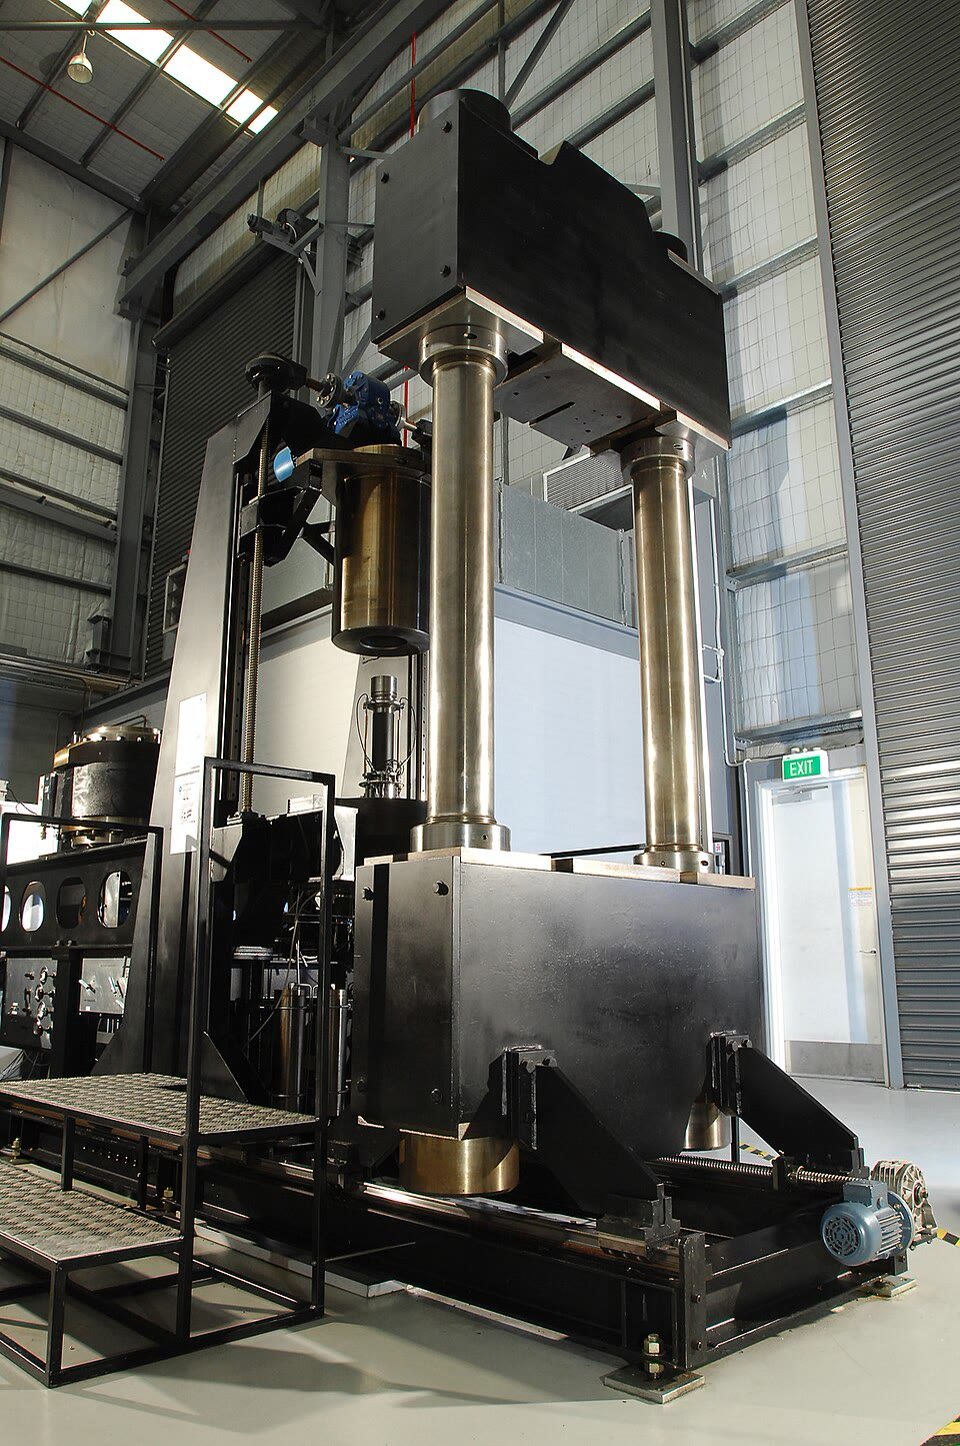
\includegraphics[width=\linewidth]{images/book3/b1-triaxial-cell.jpg}

{\scriptsize Una celda triaxial de alta presión para medir la resistencia de la roca (Darryl Peroni, CSIRO, CC BY 3.0).}
% ledger: commons:csiro-triaxial
\end{minipage}
\end{inthelab}

\section{La resistencia de la litosfera}\label{sec:b1:stress-strain-rheology:envelope}

En cada profundidad la \omterm{def:b1:layered-earth:lithosphere}{litosfera} puede fallar de dos maneras: por deslizamiento sobre fallas, con una resistencia que crece con la presión efectiva, o por
fluencia, con una resistencia que disminuye al calentarse. Se deforma de la manera que necesita el esfuerzo menor.

\begin{definition}[Envolvente de resistencia, transición frágil--dúctil, capa sismogénica]\label{def:b1:stress-strain-rheology:strength-envelope}
La \emph{envolvente de resistencia}\index{envolvente de resistencia} de la \omterm{def:b1:layered-earth:lithosphere}{litosfera} es la curva, frente a la profundidad, del mayor \omterm{def:b1:stress-strain-rheology:principal}{esfuerzo diferencial} que puede
soportar a una velocidad de deformación dada: a cada profundidad, el menor entre la resistencia por fricción y la resistencia de fluencia. La
\emph{transición frágil--dúctil}\index{transición frágil--dúctil} es la profundidad a la que ambas son iguales: por encima de ella la roca se deforma por fallamiento, por
debajo por fluencia. La \emph{capa sismogénica}\index{capa sismogénica} es el rango de profundidades en el que empiezan la mayoría de los terremotos.
\end{definition}

\begin{proposition}[Resistencia por fricción con la profundidad]\label{prop:b1:stress-strain-rheology:brittle-gradient}
En una capa de densidad $\rho$ con presión de poro hidrostática, un esfuerzo principal vertical, fallas de todas las orientaciones y sin \omterm{def:b1:stress-strain-rheology:coulomb}{cohesión}, que deslizan
con fricción $\mu$ empiezan con el \omterm{def:b1:stress-strain-rheology:principal}{esfuerzo diferencial}
\begin{align*}
  \sigma_1 - \sigma_3 &= \frac{2\mu}{\sqrt{1+\mu^2} + \mu}\,\rho g z(1-\lambda)
  && \text{si $\sigma_v = \sigma_1$}, \\
  \sigma_1 - \sigma_3 &= \frac{2\mu}{\sqrt{1+\mu^2} - \mu}\,\rho g z(1-\lambda)
  && \text{si $\sigma_v = \sigma_3$},
\end{align*}
con $\lambda = \rho_w/\rho$: el primer caso da fallas normales, el segundo cabalgamientos.
\end{proposition}

\begin{proof}
El \omterm{def:b1:stress-strain-rheology:lithostatic}{esfuerzo efectivo} vertical es $S = \rho g z - \rho_w g z = \rho g z(1-\lambda)$.
Con $C = 0$ y $k = \sqrt{1+\mu^2}$, \cref{thm:b1:stress-strain-rheology:failure-angle}
dice que una falla desliza cuando $r = \mu c'/k$, con $r$ el radio y $c'$ el
centro del círculo de Mohr efectivo. Si $\sigma_v = \sigma_1$, entonces
$\sigma_1' = S$ y $c' = S - r$, así que $rk = \mu S - \mu r$ y
$r = \mu S/(k+\mu)$. Si $\sigma_v = \sigma_3$, entonces $c' = S + r$ y
$r = \mu S/(k-\mu)$. El \omterm{def:b1:stress-strain-rheology:principal}{esfuerzo diferencial} es $2r$.
\end{proof}

Con $\mu = 0.85$ y $\rho = \qty{2700}{kg.m^{-3}}$, $S$ crece \qty{16.7}{MPa} por kilómetro y la resistencia por fricción \qty{13.1}{MPa} por kilómetro bajo
\omterm{def:b1:stress-strain-rheology:strain}{extensión} y \qty{61.3}{MPa} por kilómetro bajo compresión, casi cinco veces más: una \omterm{def:b1:layered-earth:layers}{corteza} es mucho más fácil de separar que de empujar. Más allá de un
\omterm{def:b1:stress-strain-rheology:stress}{esfuerzo normal} efectivo de \qty{200}{MPa} toma el relevo la rama superior de la \omterm{prop:b1:stress-strain-rheology:byerlee}{ley de Byerlee}, y la pendiente baja, en compresión, a unos \qty{35}{MPa} por kilómetro.
% computed in figdata/bachelor-1/strength_envelope.py (tested); ledger: byerlee:1975

\begin{omfigure}
\begin{tikzpicture}
\pgfplotsset{envaxis/.style={omrecord, omdepth, scale only axis, width=5.6cm, height=7.2cm,
  xmin=-1000, xmax=2500, ymin=0, ymax=80, xtick={-1000,0,1000,2000},
  ytick={0,10,...,80}, unbounded coords=jump,
  xlabel={esfuerzo diferencial $\sigma_1-\sigma_3$ (MPa)},
  tick label style={font=\scriptsize}, label style={font=\small},
  scaled x ticks=false, xticklabel style={/pgf/number format/.cd, 1000 sep={\,}}}}
% computed in figdata/bachelor-1/strength_envelope.py; ledger: byerlee:1975, lopez:flow-laws, codata:R, prem:moho-average
\begin{axis}[envaxis, name=cont, ylabel={profundidad (km)}, title={\small (a) continente, \qty{55}{mW.m^{-2}}}]
\addplot[fill=omLithGranite!45, draw=none] table[x=x, y=depth] {figdata/out/bachelor-1-strength_envelope-continental-outline.dat};
\addplot[omThm, line width=0.5pt, restrict x to domain=-1:2450] table[x=thrust, y=depth] {figdata/out/bachelor-1-strength_envelope-continental.dat};
\addplot[omThm, line width=0.5pt, restrict x to domain=-2450:1] table[x expr=-\thisrow{normal}, y=depth] {figdata/out/bachelor-1-strength_envelope-continental.dat};
\addplot[omDef, line width=0.5pt, restrict x to domain=-1:2450] table[x=ductile, y=depth] {figdata/out/bachelor-1-strength_envelope-continental.dat};
\addplot[omDef, line width=0.5pt, restrict x to domain=-2450:1] table[x expr=-\thisrow{ductile}, y=depth] {figdata/out/bachelor-1-strength_envelope-continental.dat};
\addplot[black, line width=1.0pt] table[x=x, y=depth] {figdata/out/bachelor-1-strength_envelope-continental-outline.dat};
\draw[black!60, dashed] (axis cs:-1000,35) -- (axis cs:2500,35);
\node[font=\scriptsize, anchor=south east] at (axis cs:2480,35) {Moho};
\draw[black, densely dotted] (axis cs:0,0) -- (axis cs:0,80);
\draw[black!70] (axis cs:660,13.7) -- (axis cs:1700,18) node[anchor=north, font=\scriptsize, align=center, text=black] {transición\\ \qty{14}{km}};
\draw[black!70] (axis cs:1870,44.6) -- (axis cs:1950,53) node[anchor=north, font=\scriptsize, align=center, text=black] {transición\\ del manto};
\node[font=\scriptsize, anchor=north, omThm] at (axis cs:1500,3) {compresión};
\node[font=\scriptsize, anchor=north, omThm] at (axis cs:-560,3) {extensión};
\node[font=\scriptsize, anchor=west, omDef] at (axis cs:40,31) {cuarzo húmedo};
\node[font=\scriptsize, anchor=west, omDef] at (axis cs:300,66) {olivino seco};
\end{axis}
\begin{axis}[envaxis, at={(cont.east)}, anchor=west, xshift=0.6cm, yticklabels={}, title={\small (b) fondo oceánico de \qty{60}{Myr}}]
\addplot[fill=omLithBasalt!45, draw=none] table[x=x, y=depth] {figdata/out/bachelor-1-strength_envelope-oceanic-outline.dat};
\addplot[omThm, line width=0.5pt, restrict x to domain=-1:2450] table[x=thrust, y=depth] {figdata/out/bachelor-1-strength_envelope-oceanic.dat};
\addplot[omThm, line width=0.5pt, restrict x to domain=-2450:1] table[x expr=-\thisrow{normal}, y=depth] {figdata/out/bachelor-1-strength_envelope-oceanic.dat};
\addplot[omDef, line width=0.5pt, restrict x to domain=-1:2450] table[x=ductile, y=depth] {figdata/out/bachelor-1-strength_envelope-oceanic.dat};
\addplot[omDef, line width=0.5pt, restrict x to domain=-2450:1] table[x expr=-\thisrow{ductile}, y=depth] {figdata/out/bachelor-1-strength_envelope-oceanic.dat};
\addplot[black, line width=1.0pt] table[x=x, y=depth] {figdata/out/bachelor-1-strength_envelope-oceanic-outline.dat};
\draw[black, densely dotted] (axis cs:0,0) -- (axis cs:0,80);
\draw[black!70] (axis cs:2003,38.2) -- (axis cs:1900,50) node[anchor=north, font=\scriptsize, align=center, text=black] {transición\\ \qty{38}{km}};
\node[font=\scriptsize, anchor=west, omDef] at (axis cs:300,66) {olivino seco};
\end{axis}
\end{tikzpicture}
\par\smallskip{\small \omterm{def:b1:stress-strain-rheology:strength-envelope}{Envolventes de resistencia} a la velocidad de deformación \qty{e-15}{s^{-1}}. Rojo: la resistencia por fricción de la \omterm{prop:b1:stress-strain-rheology:byerlee}{ley de
Byerlee} con presión de poro hidrostática, para compresión (cabalgamiento, a la derecha) y \omterm{def:b1:stress-strain-rheology:strain}{extensión} (fallamiento normal, a la izquierda, dibujada como
negativa); azul: la resistencia de fluencia de la cuarcita húmeda en la \omterm{def:b1:layered-earth:layers}{corteza} continental y del \omterm{def:b1:rock-forming-minerals:groups}{olivino} seco en el \omterm{def:b1:layered-earth:layers}{manto}; contorno negro y sombreado: la
resistencia, la menor de las dos a cada profundidad. (a) Un continente con un \omterm{def:b1:heat-budget:heat-flow}{flujo de calor} en superficie de \qty{55}{mW.m^{-2}} y una \omterm{def:b1:layered-earth:layers}{corteza} de
\qty{35}{km} de espesor: \omterm{def:b1:layered-earth:layers}{corteza} superior fuerte, \omterm{def:b1:layered-earth:layers}{corteza} inferior débil, \omterm{def:b1:layered-earth:layers}{manto} más alto fuerte. (b) Fondo oceánico de \qty{60}{Myr}: una sola capa fuerte,
de \qty{38}{km} de espesor en compresión.}
\label{fig:b1:stress-strain-rheology:envelope}
\end{omfigure}

La figura de arriba reúne las dos resistencias para dos \omterm{def:b1:layered-earth:lithosphere}{litosferas}. El continente tiene el \omterm{def:b1:heat-budget:geotherm}{geotermo} de \cref{ch:b1:heat-budget} con un \omterm{def:b1:heat-budget:heat-flow}{flujo de calor}
en superficie de \qty{55}{mW.m^{-2}}, una \omterm{def:b1:layered-earth:layers}{corteza} de cuarcita húmeda de \qty{35}{km} de espesor, y \omterm{def:b1:rock-forming-minerals:groups}{olivino} seco debajo; el fondo oceánico tiene
\qty{60}{Myr}, con el \omterm{def:b1:heat-budget:geotherm}{geotermo} del semiespacio del mismo capítulo, y \omterm{def:b1:rock-forming-minerals:groups}{olivino} desde el fondo del mar hacia abajo. La velocidad de deformación es
\qty{e-15}{s^{-1}}. Los \qty{35}{km} son la profundidad media del \omterm{def:b1:layered-earth:discontinuity}{Moho} bajo los continentes en el \omterm{def:b1:layered-earth:reference-model}{modelo de Tierra de referencia} de \cref{ch:b1:layered-earth}.
% ledger: prem:moho-average

Bajo el continente la \omterm{def:b1:stress-strain-rheology:strength-envelope}{transición frágil--dúctil} cae a \qty{13.7}{km} en compresión, a \qty{249}{\degreeCelsius}, y a \qty{17.1}{km} en \omterm{def:b1:stress-strain-rheology:strain}{extensión}. Una
\omterm{def:b1:layered-earth:layers}{corteza} más caliente la subiría, y una más fría la hundiría, ya que la ley de fluencia depende solo de la temperatura a un esfuerzo dado. La transición
es el nivel más fuerte de la \omterm{def:b1:layered-earth:layers}{corteza}.
Por debajo de ella la resistencia se desploma: en el \omterm{def:b1:layered-earth:discontinuity}{Moho}, a \qty{527}{\degreeCelsius}, la cuarcita fluye bajo \qty{7.6}{MPa}, mientras que el \omterm{def:b1:rock-forming-minerals:groups}{olivino} a la misma
temperatura necesitaría unos \qty{30000}{MPa}, tan por encima de la resistencia por fricción que la parte superior del \omterm{def:b1:layered-earth:layers}{manto} vuelve a ser frágil. Una segunda
transición sigue a \qty{44.6}{km} en compresión. La \omterm{def:b1:layered-earth:layers}{corteza} inferior de este modelo es una capa blanda entre dos fuertes: el «sándwich de gelatina». Bajo el océano
toda la \omterm{def:b1:layered-earth:lithosphere}{litosfera} es \omterm{def:b1:rock-forming-minerals:groups}{olivino}, y la resistencia crece hacia abajo hasta una sola transición a \qty{38.2}{km}, a \qty{641}{\degreeCelsius}.
% computed in figdata/bachelor-1/strength_envelope.py (tested)

Los terremotos concuerdan con la envolvente oceánica: dentro de las placas oceánicas alcanzan profundidades donde la temperatura es de \qtyrange{600}{800}{\degreeCelsius},
cerca de los \qty{641}{\degreeCelsius} de la transición única del modelo. Los terremotos más profundos solo ocurren donde una placa se hunde bajo otra, hasta más de
\qty{700}{km} (\cref{ch:b1:active-margins}).
% ledger: jackson:jelly, usgs:deepest

El \omterm{def:b1:layered-earth:layers}{manto} continental es donde el cuadro está en disputa. Durante unos veinte años el sándwich de gelatina fue la visión dominante, basada en mediciones de
laboratorio de \omterm{def:b1:rock-forming-minerals:groups}{olivino} seco y en unos pocos terremotos que se creían situados bajo el \omterm{def:b1:layered-earth:discontinuity}{Moho}. En 2002 James Jackson sostuvo que debía abandonarse: profundidades
mejor determinadas mostraron que los terremotos de los continentes se confinan a una sola capa, por lo general la \omterm{def:b1:layered-earth:layers}{corteza} superior, a veces toda la \omterm{def:b1:layered-earth:layers}{corteza}, sin
terremotos convincentes en el \omterm{def:b1:layered-earth:layers}{manto} debajo, incluso donde el \omterm{def:b1:layered-earth:discontinuity}{Moho} está solo a \qtyrange{300}{500}{\degreeCelsius}. Pequeñas cantidades de agua, unas pocas
partes por millón en el \omterm{def:b1:rock-forming-minerals:groups}{olivino}, bastan para debilitarlo drásticamente, y el \omterm{def:b1:layered-earth:layers}{manto} continental bien puede contener tanto; la resistencia de los continentes
residiría entonces sobre todo en su \omterm{def:b1:layered-earth:layers}{corteza}. Las dos visiones dibujan envolventes distintas a partir de las mismas leyes, con \omterm{def:b1:rock-forming-minerals:groups}{olivino} seco o húmedo bajo el \omterm{def:b1:layered-earth:discontinuity}{Moho}.
% ledger: jackson:jelly
Sea cual sea la correcta, una envolvente es una cota y no una medición: las leyes de laboratorio se extrapolan a lo largo de muchos órdenes de magnitud de velocidad
de deformación, y los esfuerzos máximos que muestra, más de un gigapascal, están muy por encima de los \qtyrange{1}{10}{MPa} que se observan liberar a los terremotos.
% ledger: jackson:jelly

\section{Ejercicios}

\begin{exercise}[$\star$]\label{exo:b1:stress-strain-rheology:1}
Tómese una \omterm{def:b1:layered-earth:layers}{corteza} de densidad \qty{2700}{kg.m^{-3}} y $g = \qty{9.81}{m.s^{-2}}$. A una profundidad de \qty{10}{km},
calcúlense (a) el esfuerzo vertical, (b) la presión hidrostática de poros y (c) el esfuerzo vertical efectivo y el cociente
de presión de poros $\lambda$.
\end{exercise}

\begin{exercise}[$\star$]\label{exo:b1:stress-strain-rheology:2}
(a) Una capa de \qty{10}{km} de longitud se estira hasta \qty{13}{km}: exprésense su \omterm{def:b1:stress-strain-rheology:strain}{extensión} y su elongación. (b) Otra,
de \qty{10}{km} de longitud, se acorta hasta \qty{7}{km}. (c) Dos líneas de una roca que eran perpendiculares forman ahora
un ángulo de \ang{60}: ¿cuáles son la cizalla angular y la \omterm{def:b1:stress-strain-rheology:strain}{deformación de cizalla}?
\end{exercise}

\begin{exercise}[$\star$]\label{exo:b1:stress-strain-rheology:3}
En un punto, $\sigma_1 = \qty{100}{MPa}$ y $\sigma_3 = \qty{40}{MPa}$. (a) Dibújese el círculo de Mohr. (b) ¿Cuál es el
esfuerzo de cizalla máximo, en qué planos actúa y qué \omterm{def:b1:stress-strain-rheology:stress}{esfuerzo normal} actúa sobre ellos? (c) Calcúlense $\sigma_n$ y $\tau$
en el plano cuya normal forma \ang{30} con $\sigma_1$.
\end{exercise}

\begin{exercise}[$\star$]\label{exo:b1:stress-strain-rheology:4}
Una roca tiene una \omterm{def:b1:stress-strain-rheology:coulomb}{cohesión} de \qty{10}{MPa} y un \omterm{def:b1:stress-strain-rheology:coulomb}{ángulo de fricción interna} de \ang{30}. (a) ¿A qué ángulo respecto de
$\sigma_1$ se rompe, y qué ángulo forman entre sí los dos posibles planos de fractura? (b) Con
$\sigma_3' = \qty{20}{MPa}$, ¿qué $\sigma_1'$ efectivo la rompe?
\end{exercise}

\begin{exercise}[$\star\star$]\label{exo:b1:stress-strain-rheology:5}
En los ejes $x$ (horizontal) e $y$ (vertical), $\sigma_{xx} = \qty{60}{MPa}$, $\sigma_{yy} = \qty{20}{MPa}$ y
$\sigma_{xy} = \qty{15}{MPa}$. (a) Calcúlense los \omterm{def:b1:stress-strain-rheology:principal}{esfuerzos principales} y el ángulo $\theta_p$. (b) Compruébese con
\cref{prop:b1:stress-strain-rheology:transformation} que el plano de normal $\theta_p$ no lleva esfuerzo de cizalla y que
lleva el \omterm{def:b1:stress-strain-rheology:stress}{esfuerzo normal} $\sigma_1$. (c) ¿Cuál es el esfuerzo de cizalla máximo en este punto?
\end{exercise}

\begin{exercise}[$\star\star$]\label{exo:b1:stress-strain-rheology:6}
Una zona de cizalla ha deformado su roca mediante una \omterm{def:b1:stress-strain-rheology:shear-types}{cizalla simple} $\gamma = 2$. (a) Calcúlense los estiramientos
principales y el ángulo que forma el eje largo de la \omterm{def:b1:stress-strain-rheology:strain-ellipse}{elipse de deformación} con la dirección de cizalla. (b) Compruébese que
el área no ha cambiado. (c) Una línea de material estaba a \ang{45} de la dirección de cizalla, y ascendía en el sentido de
la cizalla: ¿dónde se encuentra ahora y cuál es su estiramiento? Compárese con (a).
\end{exercise}

\begin{exercise}[$\star\star$]\label{exo:b1:stress-strain-rheology:7}
En una zona de cizalla de \qty{200}{m} de espesor, unas pequeñas manchas redondas en una pizarra se han convertido en
elipses con ejes en la proporción 4 a 1. Supóngase una \omterm{def:b1:stress-strain-rheology:shear-types}{cizalla simple}, sin cambio de área. (a) Hállense $S_1$, $S_2$ y
$\gamma$. (b) ¿A qué ángulo de las paredes de la zona deben situarse los ejes largos? (c) ¿Cuánto ha avanzado una pared
respecto de la otra?
\end{exercise}

\begin{exercise}[$\star\star$]\label{exo:b1:stress-strain-rheology:8}
Una falla a una profundidad de \qty{3}{km}, en \omterm{def:b1:layered-earth:layers}{corteza} de densidad \qty{2700}{kg.m^{-3}}, soporta un \omterm{def:b1:stress-strain-rheology:stress}{esfuerzo normal} de
\qty{70}{MPa} y un esfuerzo de cizalla de \qty{30}{MPa}. (a) Con presión hidrostática de poros, ¿desliza según la \omterm{prop:b1:stress-strain-rheology:byerlee}{ley de
Byerlee}? (b) ¿Y si los poros están sellados y $\lambda = 0.6$? (c) Hállese el valor de $\lambda$ al que empieza a deslizar.
\end{exercise}

\begin{exercise}[$\star\star$]\label{exo:b1:stress-strain-rheology:9}
Úsese la ley de fluencia del cuarcita húmeda (\cref{prop:b1:stress-strain-rheology:creep}). (a) ¿Por qué factor debe
aumentar el esfuerzo para que fluya diez veces más deprisa? (b) ¿Por qué factor disminuye su resistencia entre
\qty{400}{\degreeCelsius} y \qty{500}{\degreeCelsius}, a la misma velocidad y con $V = 0$? (c) Explíquese con estos dos
resultados por qué la profundidad de la \omterm{def:b1:stress-strain-rheology:strength-envelope}{transición frágil--dúctil} depende mucho más del geoterma que de la velocidad de
deformación.
\end{exercise}

\begin{exercise}[$\star\star\star$]\label{exo:b1:stress-strain-rheology:10}
Donde el esfuerzo vertical es $\sigma_2$, las fallas son de desgarre. Supóngase que el esfuerzo vertical efectivo es
entonces la media $(\sigma_1' + \sigma_3')/2$. (a) Demuéstrese que el deslizamiento con fricción $\mu$ y sin \omterm{def:b1:stress-strain-rheology:coulomb}{cohesión}
empieza en $\sigma_1 - \sigma_3 = 2\mu\,\rho g z(1-\lambda)/\sqrt{1+\mu^2}$. (b) Calcúlese la pendiente en megapascales por
kilómetro para $\mu = 0.85$ y $\rho = \qty{2700}{kg.m^{-3}}$, y sitúese entre las pendientes de las fallas normales e
inversas. (c) Exprésese cada una de las tres pendientes como múltiplo del esfuerzo vertical efectivo.
\end{exercise}

\begin{exercise}[$\star\star\star$]\label{exo:b1:stress-strain-rheology:11}
Modélese la \omterm{def:b1:layered-earth:lithosphere}{litosfera} oceánica de \qty{60}{Myr} como un semiespacio enfriado desde \qty{1350}{\degreeCelsius}, con una
superficie a \qty{0}{\degreeCelsius} y $\kappa = \qty{e-6}{m^2.s^{-1}}$: $T = \num{1350}\operatorname{erf}\bigl(z/(2\sqrt{\kappa t})\bigr)$.
(a) Calcúlese $2\sqrt{\kappa t}$. (b) Hállense las profundidades de las isotermas de \qty{600}{\degreeCelsius} y
\qty{800}{\degreeCelsius}. (c) Los terremotos dentro de las placas oceánicas alcanzan las profundidades donde la temperatura
está entre \qtyrange{600}{800}{\degreeCelsius}. Compárese con la \omterm{def:b1:stress-strain-rheology:strength-envelope}{transición frágil--dúctil} de la \omterm{def:b1:stress-strain-rheology:strength-envelope}{envolvente de resistencia}
oceánica de este capítulo, a \qty{38.2}{km} y \qty{641}{\degreeCelsius}.
% ledger: jackson:jelly
\end{exercise}

\begin{exercise}[$\star\star\star$]\label{exo:b1:stress-strain-rheology:12}
Una roca está atravesada por fracturas de todas las orientaciones, todas ellas con la dirección de $\sigma_2$, sin \omterm{def:b1:stress-strain-rheology:coulomb}{cohesión}
y con fricción 0.85. Los \omterm{def:b1:stress-strain-rheology:principal}{esfuerzos principales} efectivos son $\sigma_1' = \qty{110}{MPa}$ y $\sigma_3' = \qty{20}{MPa}$.
(a) Demuéstrese que algunas fracturas deslizan. (b) Hállese el intervalo del ángulo entre las fracturas que deslizan y
$\sigma_1$. ¿Cuál está en el centro del intervalo? (c) ¿Hasta qué valor de $\sigma_1'$, con $\sigma_3'$ fijo, desliza
todavía al menos una fractura?
\end{exercise}

\section{Problema: ¿deslizará la falla?}

\begin{problem}[{Problema de fin de semana --- el esfuerzo sobre una falla normal a cinco kilómetros de profundidad, su margen
de seguridad y el aumento de la presión de poros que la haría deslizar}]
\label{pb:b1:stress-strain-rheology:1}
% values: calc/ch16.py; ledger: byerlee:1975, hb81:denver
Una falla tiene \omterm{def:b1:geological-maps:attitude}{rumbo} norte--sur y buza \ang{60} hacia el este. Un pozo de inyección la alcanza a una profundidad de
\qty{5.00}{km}, en \omterm{def:b1:layered-earth:layers}{corteza} de densidad \qty{2700}{kg.m^{-3}} cuyos poros comunican con la superficie. Una medición en el
pozo da el esfuerzo horizontal perpendicular a la falla, \qty{75.0}{MPa}; el esfuerzo horizontal a lo largo del \omterm{def:b1:geological-maps:attitude}{rumbo} está
entre él y el esfuerzo vertical, así que el problema es bidimensional en el plano vertical este--oeste. Tómese
$g = \qty{9.81}{m.s^{-2}}$, agua de densidad \qty{1000}{kg.m^{-3}} y la \omterm{prop:b1:stress-strain-rheology:byerlee}{ley de Byerlee}. Dense los esfuerzos con una
precisión de \qty{0.01}{MPa}.

\medskip
\noindent\textbf{Parte I --- El estado de esfuerzos.}
\begin{enumerate}
  \item Calcúlese el esfuerzo vertical a la profundidad de la falla.
  \item Calcúlese la presión hidrostática de poros allí, y el cociente $\lambda$.
  \item ¿Cuál de los dos esfuerzos es $\sigma_1$ y cuál $\sigma_3$? ¿Qué clase de falla impulsa este estado de esfuerzos?
  \item Calcúlese el \omterm{def:b1:stress-strain-rheology:principal}{esfuerzo diferencial}, el centro y el radio del círculo de Mohr.
  \item Calcúlense los \omterm{def:b1:stress-strain-rheology:principal}{esfuerzos principales} efectivos y el centro del círculo efectivo.
  \item Con $x$ horizontal hacia el este e $y$ vertical, escríbanse las tres componentes $\sigma_{xx}$, $\sigma_{yy}$,
        $\sigma_{xy}$. ¿Por qué es nula $\sigma_{xy}$?
\end{enumerate}

\medskip
\noindent\textbf{Parte II --- Los esfuerzos sobre la falla.}
\begin{enumerate}[resume]
  \item Dese el vector unitario normal a la falla en los ejes de la pregunta 6, y el ángulo $\theta$ entre él y $\sigma_1$.
  \item Calcúlense $\sigma_n$ y $\tau$ sobre la falla con \cref{prop:b1:stress-strain-rheology:transformation}.
  \item Compruébense ambos valores con el círculo de Mohr: ¿a qué ángulo desde el extremo de $\sigma_1$ se encuentra la falla?
  \item Calcúlese el \omterm{def:b1:stress-strain-rheology:stress}{esfuerzo normal} efectivo sobre la falla.
  \item Calcúlese el cociente $\tau/\sigma_n'$ y compárese con 0.85.
  \item ¿Qué esfuerzo de cizalla haría deslizar la falla con el \omterm{def:b1:stress-strain-rheology:stress}{esfuerzo normal} efectivo actual? ¿En cuántos megapascales se queda corta?
\end{enumerate}

\medskip
\noindent\textbf{Parte III --- Círculo de Mohr y ley de Byerlee.}
\begin{enumerate}[resume]
  \item Dibújense a escala el círculo de Mohr efectivo y la recta de Byerlee.
  \item Calcúlese la distancia del centro del círculo a la recta y compárese con el radio. ¿Puede deslizar algún plano de la roca?
  \item ¿Qué plano deslizaría primero? Dense su ángulo con $\sigma_1$ y su \omterm{def:b1:geological-maps:attitude}{buzamiento}.
  \item Con \cref{prop:b1:stress-strain-rheology:brittle-gradient}, calcúlese el \omterm{def:b1:stress-strain-rheology:principal}{esfuerzo diferencial} al que deslizan las fallas
        normales a esta profundidad, y compárese con la pendiente de \qty{13.1}{MPa} por kilómetro.
  \item ¿Cuánto tendría que bajar el esfuerzo horizontal para que deslizara el plano mejor orientado?
  \item ¿Cuánto para que deslice la falla del problema? Explíquese por qué es menor.
\end{enumerate}

\medskip
\noindent\textbf{Parte IV --- Inyección.}
\begin{enumerate}[resume]
  \item Explíquese por qué un aumento $\Delta P$ de la presión de poros desplaza el círculo efectivo $\Delta P$ hacia la
        izquierda sin cambiar su radio.
  \item Calcúlese el aumento de presión de poros que lleva el plano mejor orientado a deslizar.
  \item El pozo está lleno de agua. ¿Qué presión extra debe aplicar la bomba en la boca del pozo para elevar en esa cantidad
        la presión de poros en la falla? ¿A qué altura de columna de agua equivale?
  \item Si la fricción de la falla fuera 0.6 en lugar de 0.85, ¿ya estaría deslizando? ¿Qué indica sobre su fricción que la
        falla no deslice?
  \item ¿Con qué cociente $\lambda$ desliza el plano mejor orientado?
  \item Con un decimal, en megapascales, ¿qué aumento de presión de poros hace deslizar esta falla?
\end{enumerate}
\end{problem}
